\documentclass{article}
\usepackage{amssymb}
\usepackage{graphicx}
\usepackage{natbib}
\usepackage[pdftex]{hyperref}

  \author{Driver, Timothy C.${}^{1}$ \and
    Hankin, Robin K. S.${}^{1,2}$}

  \date{${}^{1}$ Auckland University of Technology\\
    Wellesley Street, Auckland, New Zealand\\
    +64-9-9219999x5106\\
    ${}^2$ Corresponding author\\
    \texttt{hankin.robin@gmail.com}
  }

  % Tim:   ORCID 0000-0002-3184-2118
  % Robin: ORCID 0000-0001-5982-0415


  \title{Analysis of competitive surfing tournaments with generalized Bradley-Terry likelihoods}

\begin{document}



\maketitle
  
\subsubsection*{Abstract}
Here we analyse competitive surfing, specifically the 2019 Men's World Surf
League, using formal statistical methods.  We use generalized
Bradley-Terry likelihoods to assess a number of hypotheses of interest
to the surfing community.  We quantify the dominance of
the top competitors using likelihood techniques, and go on to study
the ``Brazilian storm'' phenomenon using reified entities in two ways.
Firstly we assess the supposed Brazilian preference for beach break
and point break wave types; and secondly we consider results from the
perspective of tournament theory and test for competitors modifying
their strategy in the presence of compatriot rivals.  We quantify the
evidence for these commonly assumed features of contemporary
competitive surfing and suggest further avenues of research.

keywords: Reified Bradley-Terry, surfing, competitive surfing, noncompetitive behaviour, likelihood methods, Brazilian storm
\newpage

\section{Introduction}

Surfing is a popular and growing activity in terms of both
participation and viewing \citep{warshaw2010}.  Competitive surfing
involves surfers competing against one or more other surfers in heats
lasting 30-50 minutes \citep{booth1995}.  Points are awarded on a
10-point scale: each of five judges awards points to a surfer riding a
particular wave.  The World Surf League (WSL) is the main governing
body for professional surfers \citep{wsl}.  The WSL conducts a world
tour in which the best ranked 34 surfers compete; in addition, at each
tour venue, two ``wildcard" surfers also enter the competition, who
are ignored here due to their generally poor performance.

The 2019 WSL tour saw competitive events held at eleven
different surf locations.

The typical format is as follows.  Up to four surfers---the
competitors---are in the water simultaneously, watched by up to five
judges.  Subject to surfing etiquette, competitors are free to catch a
wave at their discretion within the heat's time window.  The judges
rate each wave ride and award points to the surfer based on a range of
subjective criteria such as stylish execution and transition of
manoeuvres, but also credit elements such as the difficulty and
novelty of the performance.  The top score and bottom score among the
five judges are removed and the remaining three judges' scores are
averaged to give the final score for the surfer for that wave.  Each
surfer's aggregate score is given by the average of the two
highest-scoring waves.  The winner is the surfer with the highest
aggregate score.

Such scoring systems are designed to account for the random nature of
wave quality while reflecting competitors' abilities fairly.
Differences in wave quality between successive days mean that direct
comparison of scores between one day and another are not informative
about competitors' abilities as they are strongly dependent on details
of wave quality at the time of the competition.  However, for a
particular heat, the order statistic---that is, which competitor
scored most highly, second highest, and third---is informative about
competitors' abilities: the wave environment is common to each surfer.

We note in passing that Lemoore had a different format from the other
venues in the championship, being held in an artificial wave pool in
which every wave was essentially identical (up to a mirror
reflection).  Statistically, there were seven heats of either 2, 4, 8,
or 16 surfers.  We show below how to incorporate the information
present in such observations with the remainder of the championship
using a consistent and intuitive statistical model.

\section{Previous statistical analysis of competitive surfing}

\citet{farley2013} analyse surfing results using
one-way ANOVA techniques and report comparisons between the top 10 and
bottom 10 surfers in the 2013 World Championship Tour and conclude
that the top-ranked athletes are more consistent than the lower-ranked
group.  They report that ``to date, only a limited number of research
studies have reported on the results of competitive surfing" [p44],
and the analysis presented here fills some of this gap.

Other statistical research into competitive surfing appears to focus
on the scoring of aerial manoeuvres compared with other manoeuvres in
events.  \citet{lundgren2014}, for example,
report that aerial manoeuvres scored higher than other stunts but had
a lower completion rate, a theme we return to below.

\section{Likelihood-based systems and points-based systems}

Table~\ref{resultstable} shows the official results table from the
tour.  We see that Ferreira places first with 59740 points, Medina
second with 56475, and so on.  The overall ranking of the surfers is
determined by summing the season's points.

As in many subjective sports, points are awarded to competitors on the
basis that a better performance attracts a higher number of points.
However, such systems are difficult to analyse statistically, because
the points awarded are intrinsically arbitrary: provided that better
performances attract more points, the precise number of points awarded
does not change the competitors' behaviour.  Competitors will
endeavour to earn the maximum number of points possible, and to do
this will deliver the best performance they are able to give.

As discussed above, analysis of order statistics does not suffer from
this particular defect~\citep{aldous2017}.  Order statistics can be
analysed using a number of formal statistical methods, but here we
focus on one method that has been successfully applied in many
competitive sporting contexts: here we suggest that Plackett-Luce
likelihood functions furnish an objective and coherent method for
ranking competitors.  Further, likelihood-based methods offer one
signal advantage over points-based systems: the ability to conduct
statistically rigorous tests of meaningful nulls.

\section{The Bradley-Terry class of probability models for order statistics}

The Bradley-Terry model \citep{bradley1954} assigns non-negative
strengths $p_1,\ldots, p_n$ to each of $n$ competitors in such a way
that the probability of $i$ beating $j\neq i$ in pairwise competition
is $\frac{p_i}{p_i+p_j}$; it is conventional to normalize so that
$\sum p_i=1$.  Further, we use a generalization due to
\citep{luce1959}, in which the probability of competitor~$i$ winning
in a field of $\left\lbrace 1,\ldots, n\right\rbrace$ is
$\frac{p_i}{p_1+\cdots +p_n}$.  Noting that there is information in
the whole of the finishing order, and not just the first across the
line, we can follow \citet{plackett1975} and consider the runner-up to
be the winner among the remaining competitors, and so on down the
finishing order. Without loss of generality, if the order of finishing
were $1,2,3,4,5$ [we write $1\succ 2\succ 3\succ 4\succ5$], then a
suitable Plackett-Luce likelihood function would be

\begin{equation}\label{competitors_1_to_5_likelihood}
\frac{p_1}{p_1+p_2+p_3+p_4+p_5}\cdot
\frac{p_2}{p_2+p_3+p_4+p_5}\cdot
\frac{p_3}{p_3+p_4+p_5}\cdot
\frac{p_4}{p_4+p_5}\cdot
\frac{p_5}{p_5}
\end{equation}

and this would be a forward ranking Plackett-Luce model in the
terminology of \citet{johnson2020}.  We now use a technique due to
\citet{hankin2010,hankin2017} and introduce fictional (reified)
entities whose nonzero Bradley-Terry strength helps certain
competitors or sets of competitors under certain conditions.  The
original example was the home-ground advantage in football.  If
players (teams) $1,2$ with strengths $p_1,p_2$ compete, and if our
observation were $a$ home wins and $b$ away wins for team $1$, and $c$
home wins and $d$ away wins for team~$2$, then a suitable likelihood
function would be

\begin{equation}\label{home_ground_advantage}
\left(\frac{p_1+p_H}{p_1+p_2+p_H}\right)^a
\left(\frac{p_1}{p_1+p_2+p_H}\right)^b
\left(\frac{p_2+p_H}{p_1+p_2+p_H}\right)^c
\left(\frac{p_2+p_H}{p_1+p_2+p_H}\right)^d,
\end{equation}

\noindent where $p_H$ is a quantification of the beneficial home
ground effect.  Similar techniques have been used to account for the
first-move advantage in chess~\citep{hankin2020}, and here we apply it
to assess the supposed Brazilian preference for particular wave types.

\section{The dataset and likelihood function}

Table~\ref{rawresults} shows the first few and last few entries in the
dataset we use.  The first line shows that, at one of the heats in
WCT01 (Coolangatta, QLD), Colapinto came first, Bailey second, and
Wright came third: we write
$\mbox{Colapinto}\succ\mbox{Bailey}\succ\mbox{Wright}$.  The last line
shows that, at WCT11 (Banzai Pipeline), Ferreira came first and Medina
second: $\mbox{Ferreira}\succ\mbox{Medina}$.  We can convert this
dataset into a Plackett-Luce likelihood function but first have to
remove the wildcards and also player Vries whose maximum likelihood
strength is zero.  For the first line we would have Plackett-Luce
likelihood function as

\begin{equation}
\frac{p_\mathrm{Colapinto}}{p_\mathrm{Colapinto} + p_\mathrm{Bailey} + p_\mathrm{Wright}}\cdot
\frac{p_\mathrm{Bailey}}{p_\mathrm{Bailey} + p_\mathrm{Wright}}
\end{equation}

\noindent [observe that there is no requirement here for the strengths
  to have unit sum].  The entire dataset has a likelihood function
that incorporates all 477 lines of Table~\ref{rawresults}, but it
includes:

\begin{equation}\label{complete_likelihood_function}
\frac{
p_\mathrm{Andino}^{19}\, p_\mathrm{Callinan}^{19}\, p_\mathrm{Coffin}^{8}\ldots
}{
(p_\mathrm{Andino} + p_\mathrm{Bourez})  (p_\mathrm{Andino} + p_\mathrm{Buchan})(p_\mathrm{Bourez} + p_\mathrm{Flores} + p_\mathrm{Freestone})\ldots
}
\end{equation}


\subsection{Bradley-Terry and pairs}

Paired comparisons are particularly favourable to Bradley-Terry
because the likelihood function is exponential family and as such is
amenable to analysis via general linear models~\citep{turner2012}.
However, this is not applicable when more than two entities are
compared; and indeed here we see comparisons between three surfers
and, in the case of Jeep Surf Freshwater Pro WCT08, many more.  It
is natural to ask how much information is contained in the
observations where more than two surfers are in the water.

We can directly calculate the determinant of the observed information
matrix for the likelihood function in
equation~\ref{complete_likelihood_function} at about $4.3\times
10^{71}$, as compared with~$2.9\times 10^{69}$ for the pairs
considered in isolation, a ratio of about $146.4$.  This ratio shows
that there is considerable information loss in considering only the
paired comparisons.  We are thus motivated to consider the whole
dataset, not just the part which involves paired comparisons.

\section{Results}

Figure~\ref{piechartmax} shows the maximum likelihood estimate for the
23 competitors' strengths, which appears to show a wide range from
Florence at about 17.5\% down to Coffin at about 1.5\%.  The {\tt
  hyper2} software~\citep{hankin2017} may be used to formally assess
one plausible null: that the competitors all have equal skill, that is
$H_0\colon p_\mathrm{Andino} = p_\mathrm{Bourez}=\ldots=
p_\mathrm{Wright}=\frac{1}{23}$, and any differences in placings are
due to random variation.  The Method of Support \citep{edwards1992}
rejects the null (in favour of the evaluate) at $p=4\times 10^{-5}$.
There is thus strong evidence to suggest that the competitors are
indeed of different skills and the result actually reflects genuine
differences in abilities, rather than the result of random chance.
Alternatively, we may view the dataset as being sufficiently
informative to reveal actual differences in surfing ability.  Observe
that the competitors' points (that is, the final column of
table~\ref{resultstable}) cannot be used for this type of
probabilistic analysis: the points awarded are arbitrary and changing
the points system would change the points scored but not affect the
competitors' behaviour.

However, points awarded may be compared with likelihood estimates, and
one would expect high points totals to be associated with high
likelihoods.  Figure~\ref{compare_likelihood_points} shows a loose
correlation ($R^2=0.64$; $p=3\times 10^{-6}$) and
Figure~\ref{compare_likelihood_points_rankings} shows how the rankings
differ when calculated by the points and likelihood systems.  Note the
anomalous position of Florence, who did not compete in five venues due
to injury: this strongly affecting his points total but not his
likelihood-based ranking.

We may ask whether the top two officially ranked competitors, Medina
and Ferreira, have different strengths.  To test the null of equal
strength, we maximize the likelihood subject to the null, and compare
with the global maximum likelihood~\citep{hankin2010}.  This gives us a
support difference of about 0.05, well short of Edwards's 2 units of
support criterion.  Alternatively, we could observe that the
$-2\log\left(\frac{\Lambda}{\Lambda_0}\right)\simeq 0.1$ is not in the
tail region of its asymptotic $\chi^2_1$ distribution.  We may thus
assert that there is no strong evidence for Ferreira's actually having
a competitive advantage over Medina.  We may similarly wonder whether
Medina is equal in strength to Wilson; here we reject the null with
support difference of about 2.33, corresponding to a $p$-value of
$0.031$.

\section{The Brazilian storm}

In surfing lore, the ``Brazilian storm'' refers to the emergence of
Brazil as a dominant nation of elite surfers.  The term was first used
to describe the fact that six out of eight quarterfinalists at the 2011 Nike
Lowers Pro were Brazilian; it rose in public consciousness following
the victories of Medina and de Souza in the World Surf League
championships in 2014 and 2015 respectively.  The storm shows no signs
of abating, with commentators such as Douglas opining that this
generation ``represents a seismic shift for Brazilian competitors onto
an entirely new plane'' \citep{douglas2020}.

Here, we study two aspects of this sporting phenomenon: the suggested
Brazilian preference for beach break and point break wave types; and the
noncompetitive effect of compatriot rivalry.

\subsection{Brazilian wave type preferences}

The statistical method described here can test many different
hypotheses inspired by surfing lore.  For example, one frequent
suggestion~\citep{burgess2020,ho2021} is that Brazilian surfers tend to
have skillsets that favour point and beach break wave types, readily
accessible to these surfers' native Brazil; see~\citet{scarfe2003} for
a scientific overview of surf break characteristics,
and~\citet{butt2004} for a surfer's perspective.

We now assess the null that Brazilians perform equally well on all
types of wave types.  To that end, we create a reified surfer,
``Brazilian wavetype", whose strength helps all Brazilian surfers
when surfing on their (putative) preferred wave type, an analogue of
the ``home ground monster" who helps the home team as per
equation~\ref{home_ground_advantage}.  Here we modify the likelihood
function only when a single Brazilian is in the water, thus avoiding
possible interaction with the compatriot issue discussed in
section~\ref{compatriot}.  The null would be that this reified entity
has zero strength.  We fail to reject this null (differential support
= 0.035; $p=0.79$) and conclude that there is no evidence to suggest
that Brazilians' performance is better on their preferred wave types
than one would expect by chance.  We may go further using the method
of support: not only is the maximum likelihood estimate for Brazilian
wavetype very small (about 0.002), but in addition we may reject the
the proposal that the strength of this entity exceeds about 0.025
(Figure~\ref{brazilian_wavetype_support}).

\section{Differential \label{compatriot} behaviour toward compatriotic competitors}

One measure of the rising popularity of surfing is its inclusion in
the 2020 Summer Olympics~\citep{tulloch2019}, and it is natural to ask
whether this would affect the competition in some way~\citep{ho2021}.
One suggestion would be that competitors become more focussed on
beating compatriots than surfers from other countries, the thinking
being that admission to a country's Olympic team would be of more
importance to a competitor than their overall standing in the
tournament.  One might expect competitors to value their ranking when
restricted to within their country more than their international
ranking.  If this is the case then we would expect competitors to
change their behaviour if they are in the water with another surfer of
the same nationality.  Specifically, if we have three surfers in the
water of whom two are of one nationality and the third of another, we
would expect the compatriots to adopt a style calculated to beat their
countryman, possibly at the expense of performance relative to the odd
man out.  In this context, risk sensitivity is likely to be become
important.  One example might be aerial manoeuvres which are risky
but, if successful, attract high scores~\citep{lundgren2014}.  Such
strategies are known to occur in chess~\citep{hankin2020}: players
suffering a sequence of defeats adopt a high-risk (all-or-nothing)
approach, while players in a winning streak hunker down, play
defensively, and entrench their lead.  Such hypotheses are difficult
to test with conventional techniques as the competitors' strengths
themselves are nuisance parameters~\citep{basu1977}.

Consider, as an example, the case of Smith, Buchan, Freestone who were
simultaneously in the water at Bells Beach, Australia.  Now, Buchan
and Freestone are Australian, and Jordy Smith is South African.  It is
reasonable to ask whether Buchan and Freestone, who are in direct
competition with one another for a place in the Australian Olympic
surfing team, would be more motivated to beating each other than to
come ahead of Smith.  This would be a rational response, but arguably
noncompetitive.  How would such a strategy manifest itself in
scorelines?  We would suggest that Smith is able to modify his
strategy to benefit from the mutual rivalry between Buchan and
Freestone; and indeed we see Smith winning that particular heat.  We
tentatively interpret this as a Nash-type equilibrium: there is no
incentive for either Buchan nor Freestone to deviate from their
prioritization of defeating their compatriot; and indeed neither
Buchan nor Freestone were selected for the 2020 Olympic team.

The reified Bradley-Terry technique furnishes an intuitive statistical
test for such mechanisms, that automatically controls for competitors'
strengths.  Noting
that the compatriots effectively place themselves at a {\em
  disadvantage} when compared with the odd man out, we introduce a
compatriot monster whose strength $p_C$ helps the odd man out.
Writing $p_1, p_2$ for the strengths of the compatriots and $q$ for
the odd man out, we construct likelihood functions for the six
possible orderings when two compatriots and an odd man out are in the
water at the same time in Table~\ref{likelihoodcompatriot} (if we have
either three different nationalities or three identical nationalities,
we revert to the standard Plackett-Luce likelihood).  Note that all
six likelihood functions in table~\ref{likelihoodcompatriot} are
informative about $p_1,p_2,q$ in addition to being informative about
the object of inference, $p_C$.

We can now apply the Method of Support to the hypothesis that $p_C=0$,
that is, that such noncompetitive behaviour is absent.  We find that
the maximum likelihood estimate for $p_C$ is about 0.015, weaker than
the ``real'' surfers, but the support for a nonzero $p_C$ is about
0.59 [asymptotic $p=0.28$], insufficient to reject our null.  We
conclude that there is no strong evidence to suggest that such
noncompetitive behaviour occurred---at least not from the order
statistics we considered.

\section{Conclusions and further work}

We analysed results from the 2019 World Surf League using reified
Bradley-Terry likelihoods to assess a number of hypotheses of interest
to the surfing community.  Reified Bradley-Terry allows the use of
formal statistical methods in ways that analysing points scored does
not.  For example, we can be confident that the results reflect
differences in skill (rather than random variation); there is no
statistical difference in strength between the top two officially
ranked competitors, Medina and Ferreira; but we may reject the
hypothesis that Medina and Wilson are equal in strength.

We discuss and assess the ``Brazilian storm'' phenomenon using reified
Bradley-Terry techniques, and show that there is no strong evidence to
support the supposed Brazilian preference for point and beach break
beaches.  We also find no evidence to suggest that surfing's being
included in the 2020 Summer Olympics results in modified strategies to
bolster intranational ranking at the expense of WCT performance.

Further work might include incorporation of more tournament results
into our likelihood function, and possibly to investigate priority
infringements between compatriots.

\bibliographystyle{agsm}
\bibliography{chess}

\clearpage
\newpage


\begin{table}[h]
\begin{tabular}{llllllllllllll}
competitor  & nationality&WCT01  &WCT02  &WCT03  & \ldots &WCT09&WCT10&WCT11&points\\ \hline
 Ferreira   &   BRA      &   1   &   5   &   17  & \ldots      &  2   &   1   &   1   &   59740\\
 Medina     &   BRA      &   5   &   5   &   17  & \ldots      &  9   &   9   &   2   &   56475\\
 Smith 	    &   ZAF      &   3   &   3   &   17  & \ldots      &  9   &   2   &   17  &   49985\\
 Toledo     &   BRA      &   9   &   2   &   5   & \ldots      &  17  &   5   &   17  &   49145\\
 Andino     &   USA      &   2   &   17  &   5   & \dots       &  5   &   5   &   9   &   46655\\
 $\ldots$   &            &   &   &       &       & \dots       &      &       &       &
\end{tabular}
\caption{Conventional league table for the top five competitors in WCT
  2019 tour. \label{resultstable} Thus at WCT01 (Coolangatta, QLD) we see
  Ferreira coming first, Andino second and Smith third}
\end{table}

\clearpage
\newpage


\begin{table}[h]
\begin{verbatim}
WCT01 Colapinto Bailey Wright
WCT01 Freestone Lau Smith
WCT01 Dora Ferreira Slater
WCT01 Duru Toledo Ibelli
WCT01 Moniz Heazlewood Wilson
...
WCT11 Medina Florence
WCT11 Colapinto Bourez
WCT11 Ferreira Slater
WCT11 Medina Colapinto
WCT11 Ferreira Medina
\end{verbatim}
\caption{Extract from observations: raw results\label{rawresults} from
  WCT 2019.  Thus the first heat at WCT01 (Coolangatta, QLD) shows
  competitors Colapinto, Bailey, and Wright in the water at the same
  time, the competition order being
  $\mbox{Colapinto}\succ\mbox{Bailey}\succ\mbox{Wright}$; as discussed
  in the text we use only the competition order for our likelihood
  function}
\end{table}

\clearpage
\newpage

\begin{table}[h]
\begin{tabular}{l|l}
order  & ${\mathcal L}(p_1,p_2,q,p_C)$\\ \hline
$p_1\succ p_2\succ q $ & $ \frac{p_1}{p_1+p_2+q+p_C}\cdot\frac{p_2}{p_2+q+p_C}$\\
$p_2\succ p_1\succ q $ & $ \frac{p_2}{p_1+p_2+q+p_C}\cdot\frac{p_1}{p_1+q+p_C}$\\
$p_1\succ q\succ p_2 $ & $ \frac{p_1}{p_1+p_2+q+p_C}\cdot\frac{q+p_C}{p_2+q+p_C}$\\
$p_2\succ q\succ p_1 $ & $ \frac{p_2}{p_1+p_2+q+p_C}\cdot\frac{q+p_C}{p_1+q+p_C}$\\
$q\succ p_1\succ p_2 $ & $ \frac{q+p_C}{p_1+p_2+q+p_C}\cdot\frac{p_1}{p_1+p_2}$\\
$q\succ p_2\succ p_1 $ & $ \frac{q+p_C}{p_1+p_2+q+p_C}\cdot\frac{p_2}{p_1+p_2}$\\
\end{tabular}
\caption{The \label{likelihoodcompatriot} six possible finishing
  orders (``$\succ$'' means ``scored more points than'') for the case
  where two compatriot surfers and an odd man out are in the water at
  the same time, with associated likelihood function for strengths
  $p_1,p_2,q, p_C$.  Here $p_1,p_2$ are the strengths of two
  compatriot surfers, $q$ the strength of the odd man out, $p_C$ the
  strength of the compatriot monster. and nationality and a third are
  in the water at the same time}
\end{table}

\clearpage
\newpage

\begin{figure}[h]
\includegraphics[width=4in]{showsurfingmaxppie.pdf} % Pie chart of strengths
\caption{Pie chart\label{piechartmax} showing maximum likelihood strengths of the 23 competitors.  Note the
dominance of Ferreira, Florence, and Medina}
\end{figure}

\clearpage
\newpage

\begin{figure}[h]
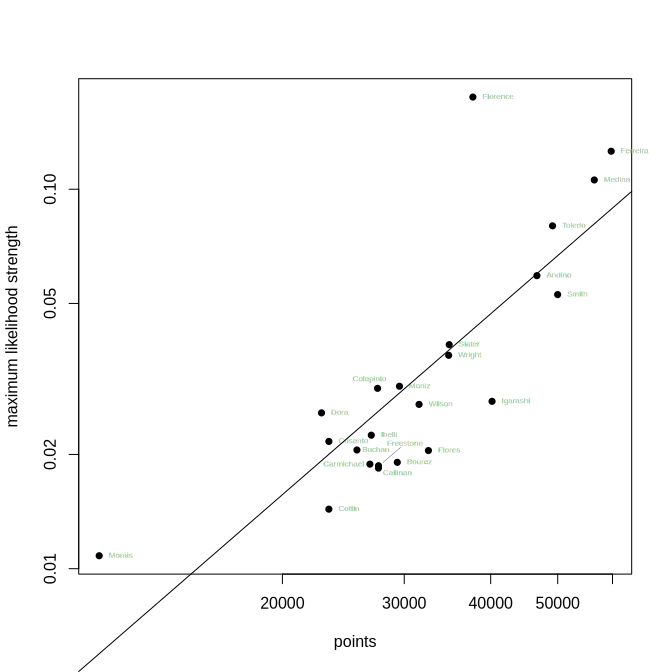
\includegraphics[width=4in]{directlogplotofstrengths.pdf}
\caption{Scatterplot of points scored  \label{compare_likelihood_points}
against maximum likelihood estimates}
\end{figure}

\clearpage
\newpage

\begin{figure}[h]
\includegraphics[width=4in]{ordertransplotplot.pdf}
\caption{Scatterplot of ranks \label{compare_likelihood_points_rankings} of points-based ranking
against likelihood-based ranking.  Note the anomalous position of
Florence}
\end{figure}

\clearpage
\newpage

\begin{figure}[h]
  \includegraphics[width=4in]{plotwidep.pdf}
\caption{Profile support \label{brazilian_wavetype_support} for the
  Brazilian wavetype reified entity.  The horizontal axis specifies a
  particular strength for Brazilian wavetype, and the height of the
  curve gives the support conditional on the x-axis}
\end{figure}

\end{document}
